سوال ۱


برای هر کدام از زبان‌های منظم زیر، یک ماشین متناهی قطعی طراحی می‌کنیم که رشته‌های آن زبان را بپذیرد.

\subsection*{۱.۱.۱}

فرض می‌کنیم 
$$N = (Q, \Sigma, \delta, q_0, F)$$
یک DFA با شرایط زیر باشد:
\begin{align*}
	Q &= P(\Sigma)\\
	\Sigma &= \{p,q,r,s\} \\
	\delta(q,a) &= q \cup a \\
	q_0 &= \{\} \\
	F &= \{q \mid |q| \neq 4\}
\end{align*}
درستی این DFA از تعریف آن آشکار است. بدین شکل که آن همه‌ی رشته‌های قابل تعریف روی الفبای مذکور را که هر کدام فاقد دست کم یکی از این کاراکترها هستند، خروجی می‌دهد.

\subsection*{۲.۱.۱}

فرض می‌کنیم 
$$N = (Q, \Sigma, \delta, q_0, F)$$
یک DFA با شرایط زیر باشد:
(در این‌جا $\pi(q)$ مجموعه‌ی همه‌ی جایگشت‌های رشته‌ی $q.$ می‌باشد.)
\begin{align*}
	Q &= \{(?, ?, ?, ?) | ? \in \{a, b, c, .\}\} \\ 
	\Sigma &= \{a,b,c\} \\
	\delta(q, a) &= \begin{cases}
		q & |q| = 4 \land q \notin F  \\
		q \ll a & O.w
	\end{cases} \\ 
	q_0 &= \{., ., ., .\} \\
	F &= \{q \mid q \notin B\} \\
	B &= \{(bbbb), (abba), (cbbc), (acba), (abca), (cabc), (cbac)\} \\ &\cup \pi(bbba) \cup \pi(bbbc)\cup \pi(bbac)
\end{align*}

\subsection*{۲.۱}

از استقرا استفاده می‌کنیم برای اثبات این بخش. در ابتدا پایه‌ی استقرا را تعریف کرده و سپس گام استقرا را اثبات می‌کنیم تا اثبات تکمیل شود. این‌جا روی طول
$\omega$
استقرا می‌زنیم.
پایه‌ی استقرا: فرض می‌کنیم طول $\omega$ صفر است. در نتیجه با توجه به تعریف، داریم:
\begin{align*}
	\hat{\delta}^{*}(q_0, \epsilon) &= \{q_0\} \\
	\delta^{*}(\{q_0\}, \epsilon) &= \{q_0\} \\
	\implies \hat{\delta}^{*}(q_0, \epsilon) &= \delta^{*}(\{q_0\}, \epsilon)
\end{align*}
حالا فرض می‌کنیم برای $\omega = \omega_1\omega_2\dots\omega_k$ نیز درست باشد. پس داریم:
\begin{align*}
	\hat{\delta}^{*}(q_0, \omega_1\dots\omega_k) &= \delta^{*}(\{q_0\}, \omega_1\dots\omega_k) \\
	\hat{\delta}^{*}(q_0, \omega_1\dots\omega_{k+1}) &= \hat{\delta}(\hat{\delta}^{*}(q_0, \omega_1 \dots \omega_{k}), w_{k + 1}) = \bigcup_{r \in \hat{\delta}^{*}(q_0, \omega_1 \dots \omega_{k})} \hat{\delta}(r, w_{k + 1})
	\\ \delta^{*}(\{q_0\}, \omega_{1}\dots\omega_{k + 1}) &= \delta(\delta^{*}(\{q_0\}, \omega_1 \dots \omega_{k}), \omega_{k+1}) = \bigcup_{r \in \delta^{*}(\{q_0\}, \omega_1 \dots \omega_{k}))} \hat{\delta}(r, w_{k + 1}) \\
	\implies \hat{\delta}^{*}(q_0, \omega_1\dots\omega_{k + 1}) &= \delta^{*}(\{q_0\}, \omega_1\dots \omega_{k+1}) \blacksquare
\end{align*}
در نتیجه اثبات کامل است.

\subsection*{۳.۱}

در این بخش کافی‌ست برای هر یک از موارد گفته شده، یک مثال نقض آوریم. یک ماشین ساده‌ی دو استیتی را نیز اگر در نظر بگیریم می‌توانیم رد کنیم موضوع مطرح شده را.

در مثال زیر، ماشین M به صورت 
$$M = (Q, \Sigma, \delta, q_0, F)$$
می‌باشد.
\\
\\
\begin{center}
	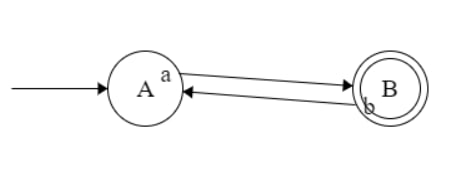
\includegraphics{DFA1}
	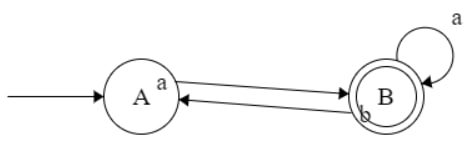
\includegraphics{DFA2}
\end{center}
در ماشین بالا ابتدا رشته‌های به فرمت
$a\{ba\}*$
را می‌پذیریم. اگر از یکی دو روش گفته شده استفاده کنیم، ماشین پایینی بدست می‌آید. این ماشین رشته‌های به فرمت
$a\{ba\}*a*$
را می‌پذیرد، همچنین رشته‌های اشتباهی نیز می‌پذیرد مانند $aaaaba$؛ پس این روش‌ها حتما درست کار نمی‌کنند و مثال نقض زدیم.

برای حالت بعدی نیز داریم که ماشین N به صورت 
$$N = (Q, \Sigma, \delta, q_0, F)$$
می‌باشد.
در این ماشین، رشته‌های به فرمت $b\{ab\}*$ پذیرفته می‌شوند. حالا اگر به روش گفته شده در شرح سوال، یال اضافه کنیم، رشته‌های به فرمت 
$a*b\{ab\}*$
را هم می‌پذیریم، اما برای مثال رشته‌ای مانند $baaaab$ را هم می‌پذیریم که مثال نقض است و در نتیجه روش گفته شده لزوما درست کار نمی‌کند.
\\
\\
\begin{center}
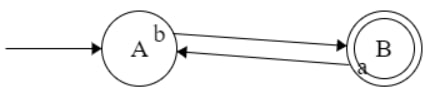
\includegraphics{DFA4}
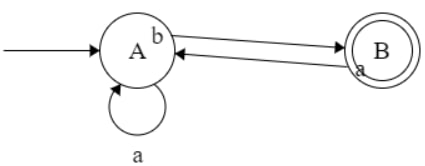
\includegraphics{DFA3}
\end{center}

